\clearpage{\pagestyle{empty}\cleardoublepage}

\chapter{Searches for vector-like top partner pairs in the single lepton channel}~\label{chap:vlq}

Starting from this chapter, and continuing in Chapter~\ref{chap:wbx} 
and Chapter~\ref{chap:htx}, we are going to describe two 
searches for vector-like top partners \TTbar\ pairs performed in the single 
lepton\footnote{In the following, with the word ``lepton'' we will 
refer either to an electron or a muon, assumed to come from the leptonic
decay of a $W$ boson or a leptonic $\tau$ decay.}
%with its associated neutrino, which is considered to be the only particle contributing to the transverse missing energy \met.}
 channel. These analyses
are optimized for different final states and are thus complementary.
The analyses are performed using a partial dataset of the pp collisions at the \cme\ 
of \rts=8~\tev\ collected during 2012 at the ATLAS detector, corresponding to an integrated luminosity of  14.3~\ifb.
The first search focuses on  vector-like top partners decay channels with high 
Branching Ratio (BR) to 
a $W$ boson and a bottom quark, while the second search is optimized for events with 
high BR to a Higgs boson and a top quark.
%and is performed using the full dataset of pp collisions at the \cme of \rts=8~\tev\ collected during 2012 at the ATLAS detector, consinsting in 20.34~\ifb, while
%search for vector-like top partners with high BR to $Ht$
%uses a partial dataset of the same data, amounting to 14.3~\ifb.

This chapter is devoted to the presentation of the general features that are common to 
the two analyses and is organized as follows: first in Section~\ref{sec:strategy}
we review the strategy for vector-like quark searches adopted 
by the Exotics group of the ATLAS collaboration; Section~\ref{sec:presel}
summarises the common event preselection for data and few general concepts in the
analyses design; Section~\ref{sec:datasets}
describes the Monte Carlo samples used in the searches, which
are in general common to both analyses with only few exceptions that are reported,
and how the multi-jet background from QCD events is
obtained; Section~\ref{sec:systematics} introduces the general treatment of systematic uncertainties.
%The two analyses are then presented in details in Chapter~\ref{chap:wbx} 
%(\TTbar\ pairs decaying to \wbx\ ) and in Chapter~\ref{chap:htx}
%(\TTbar\ pairs decaying to \htx\ ). The final results are presented 
%in Chapter~\ref{chap:results}.

\section{General strategy for vector-like quark pairs searches}\label{sec:strategy}

The phenomenology for vector-like quarks was described already in Section~\ref{sec:THvlq}
of this dissertation. Here we will only briefly re-introduce the concepts on which
the strategy for the searches has been built. Table~\ref{tab:vlqdecays} collects the 
decay modes for vector-like quarks in the singlet and doublet models. It is evident
from the richness of the final state phase space, combined with the unpredicted mass
of the heavy objects that could span from few hundreds of \gev s (down to the values exluded by
previous searches) up to  $\sim 1$~\tev\ (since we focus on pair production of vector-like
quarks, which is favoured up to this mass scale)% as shown in Figure~\ref{fig:vlqxsec}), 
that is impossible to cover it with a single inclusive search.

\begin{table}[htb]\centering
\begin{tabular}{|lc|lc|}\toprule
\hskip2ex VLQ &  Decay & \hskip2ex VLQ  & Decay \\ 
\hskip1ex Singlets &  modes & \hskip1ex Doublets & modes\\
& & &\\
$T(+2/3)$ & $W^+b,\, Ht,\, Zt$ & \multirow{2}{*}{$\quad\bigg(\begin{array}{c}T \\ B\end{array}\bigg)$} & $W^+b,\, Ht,\, Zt$\\ 
& & & $ W^-t,\, Hb,\, Zb$\\
$B(-1/3)$ & $ W^-t,\, Hb,\, Zb$ & & \\
& & \multirow{2}{*}{$\quad\bigg(\begin{array}{c}T \\ X\end{array}\bigg)$} & $Ht,\, Zt$\\
$X(+5/3)$ & $W^+t$ & & $W^+t$\\
& & &\\
$Y(-4/3)$ & $W^-b$ & \multirow{2}{*}{$\quad\bigg(\begin{array}{c}B \\ Y\end{array}\bigg)$} & $Hb,\, Zb$\\
& & & $W^-b$\\\bottomrule
\end{tabular}
\caption{Allowed decay modes for vector-like singlets and doublets.}\label{tab:vlqdecays}
\end{table}

%\begin{figure}[htb]\begin{center}
%	\subfigure{
%  	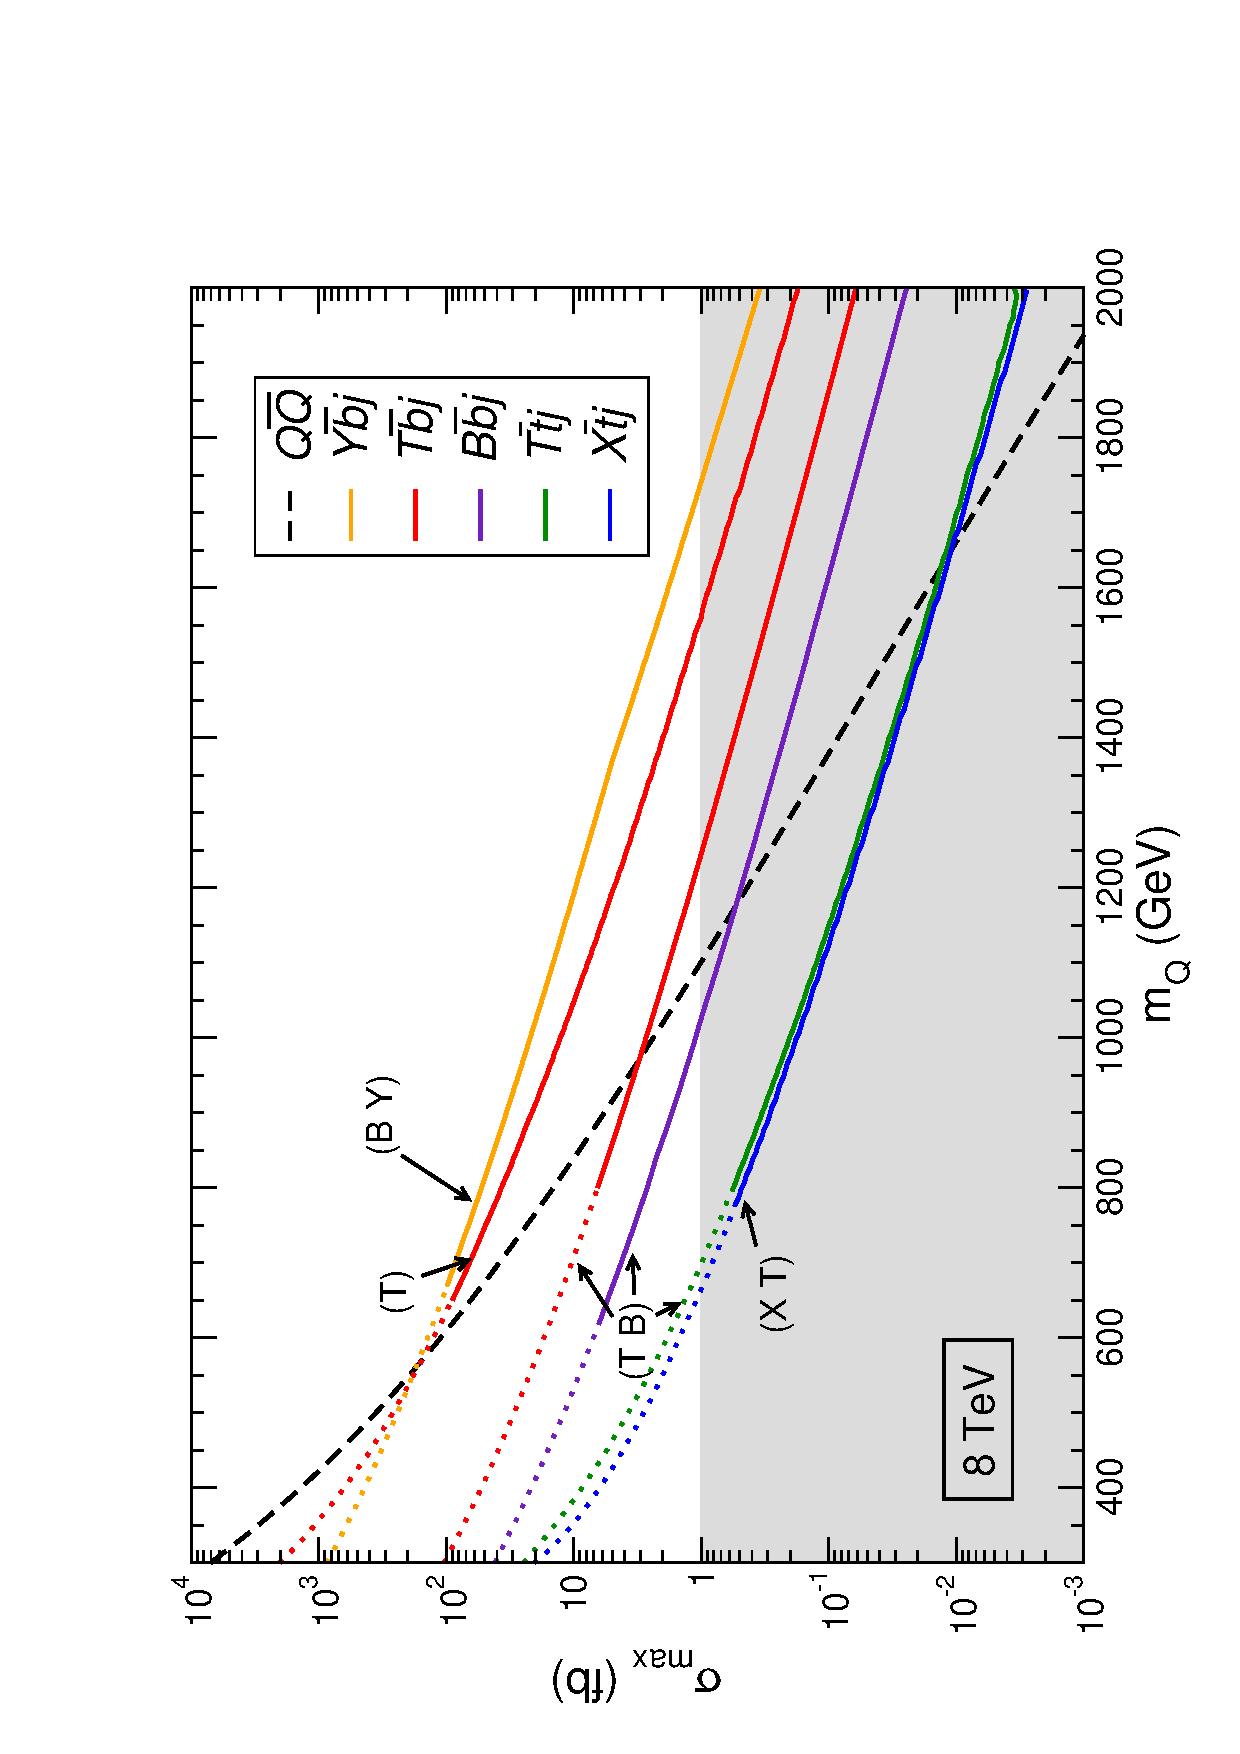
\includegraphics[width=0.65\textwidth, angle=270]{vlq_analysis/figures/xsec-8}}
%	\caption{\label{fig:vlqxsec} Pair and single production cross sections  for heavy 
%        quarks in proton-proton collisions at $\sqrt{s}=8$~TeV~\cite{Aguilar-Saavedra:2013qpa}.}
%\end{center}\end{figure}

The BR of vector-like top and bottom partners to the allowed decay modes depends
on the mass of the heavy quark and on the considered model (in our case, singlet or doublet
scenario), as shown in Figure~\ref{fig:vlqBRs}.
Each decay mode has specific features that allow to define powerful, optimized searches.
Therefore in order to exploit this opportunity and at the same time stay as model independent
as possible, different searches for vector-like quarks are performed at ATLAS
to be later combined, each of them sensitive to specific channels.
To ensure a comprehensive coverage of the phase space, a two-dimensional plane is defined 
(Figure~\ref{fig:2dplane}) as follows:
along the Y axes is the BR of the decay 
modes with a Higgs boson in the final state; along the X axis is the BR 
of the decay modes with a $W$ boson in the final state.
The BR to the channel with a $Z$ boson in the final state is then fixed by the 
unitarity requirement BR($T/B\to  Zt/b$) = 1 - BR($T/B\to Ht/b$) - BR($T/B\to Wb/t$).
A plane of this kind is defined for every vector-like quark mass point considered 
in the analysis. Each point of each plane therefore represents a 
uniquely defined model, and analyses are performed for every configuration
to either find deviations from expectations or to set a 95\% Confidence Level (CL) exclusion.
The final objective of the joint strategy is to cover the full plane by combining
analyses probing the different signatures.

\begin{figure}[h!tb]\begin{center}
	\subfigure[]{\label{fig:vltBRs}
  	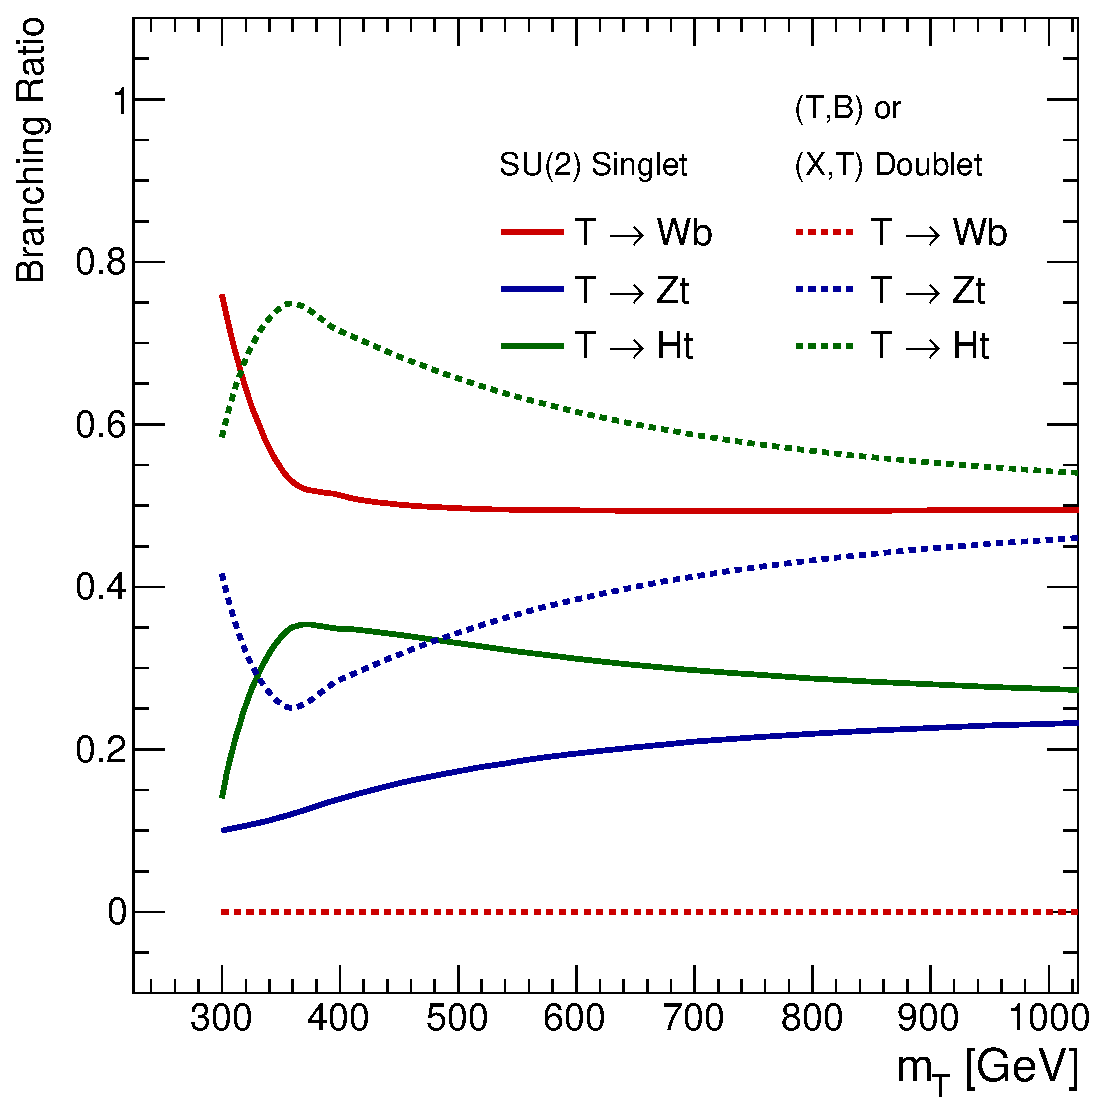
\includegraphics[width=0.47\textwidth]{vlq_analysis/figures/fig_02a.eps}}
	\subfigure[]{\label{fig:vlbBRs}
  	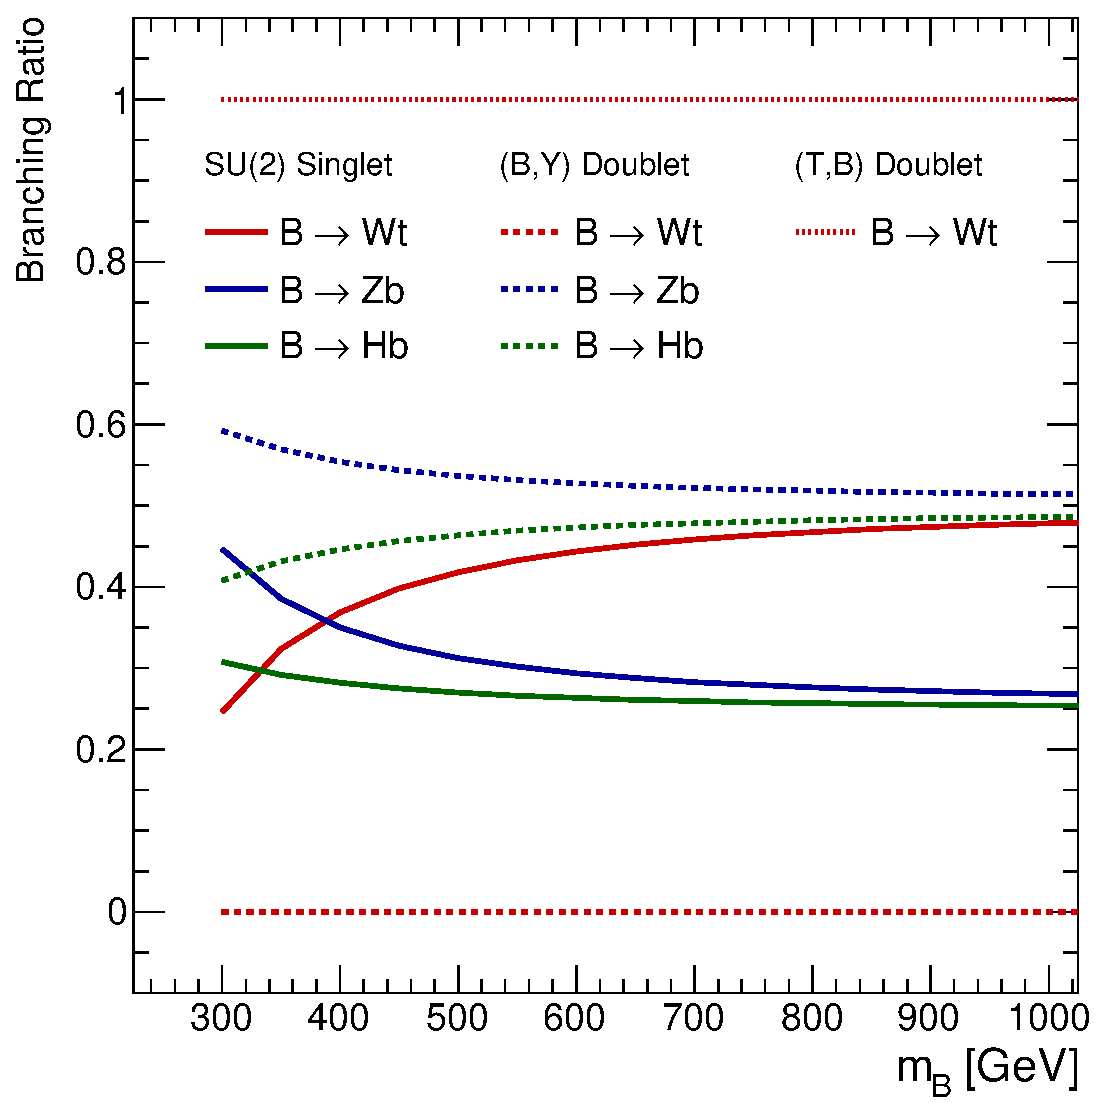
\includegraphics[width=0.47\textwidth]{vlq_analysis/figures/fig_02b.eps}}
	\caption{Branching ratio of vector-like top (a) and bottom (b) partners as a function of the heavy quark mass $m_T$ and $m_B$ respectively~\cite{ATLAS-CONF-2013-056} for singlet and doublet models.\label{fig:vlqBRs}}
\end{center}\end{figure}

\begin{figure}[h!bt]\begin{center}
	\subfigure{
        \begin{pgfpicture}{0.0\textwidth}{0.0\textheight}{.5\textwidth}{.5\textwidth}
%\begin{pgfpicture}{0.0\textwidth}{0.0\textheight}{1.\textwidth}{.6\textwidth}

\begin{pgfscope}
\pgfsetendarrow{\pgfarrowlargepointed{6pt}}
\pgfsetlinewidth{1.5pt}

\begin{pgftranslate}{\pgfpoint{0.05\textwidth}{0.05\textheight}}
%\begin{pgftranslate}{\pgfpoint{0.1\textwidth}{0.15\textheight}}
  {
    %\color{black}
    \color{black!50!red}
    \pgfputat{\pgfxy(3.5,-0.5)}{\pgfbox[left,base]{BR($T\to Wb$)}}
  }
  {
    \color{black!50!blue}
    \pgfputat{\pgfxy(3.5,-0.8)}{\pgfbox[left,base]{BR($B\to Wt$)}}
  }
  {
    \begin{pgfrotateby}{\pgfdegree{90}}
      {
        \color{black!50!red}
        \pgfputat{\pgfxy(3.5,0.4)}{\pgfbox[left,base]{BR($T\to Ht$)}}
      }
      {
        \color{black!50!blue}
        \pgfputat{\pgfxy(3.5,0.7)}{\pgfbox[left,base]{BR($B\to Hb$)}}
      }
    \end{pgfrotateby}
  }
  {
    \pgfsetlinewidth{1.5pt}
    \color{gray!30!white}%\color{light-gray}
    \pgfmoveto{\pgfxy(5,0)}
    \pgflineto{\pgfxy(5,5)}
    \pgflineto{\pgfxy(0,5)}
    %\pgfstroke
    \pgffill
  }
  {
    %\color{black}
    \pgfputlabelrotated{0.5}{\pgfxy(0,5)}{\pgfxy(5,0)}{8pt}{\pgfbox[center,base]{Forbidden}}
  }
  \begin{pgfscope}
    \pgfmoveto{\pgfxy(5,0)}
    \pgflineto{\pgfxy(0,0)}
    \pgflineto{\pgfxy(0,5)}
    {
      \color{yellow!30!white}
      \pgfclip
      \pgfcircle[fill]{\pgfxy(.5,4)}{35pt}
    }
    {
      \pgfputat{\pgfxy(0.15,3.6)}{\pgfbox[left,base]{\large{\color{black!70!red}$Ht$}{\color{black!70!blue}$(b)$}}}
    }
    {
      \color{yellow!30!white}
      \pgfcircle[fill]{\pgfxy(.6,.6)}{35pt}
    }
    {
      \pgfputat{\pgfxy(0.15,.4)}{\pgfbox[left,base]{\large{\color{black!70!red}$Zt$}{\color{black!70!blue}$(b)$}}}
    }
    {
      \color{yellow!30!white}%\color{light-gray}
      \pgfcircle[fill]{\pgfxy(4,0)}{35pt}
    }
    {
      \pgfputat{\pgfxy(3.2,0.4)}{\pgfbox[left,base]{\large{\color{black!70!red}$Wb$}{\color{black!70!blue}$(t)$}}}
    }
  \end{pgfscope}
  {
    %\color{black}
    \pgfsetendarrow{\pgfarrowlargepointed{6pt}}
    \pgfsetlinewidth{1.5pt}
    \pgfline{\pgfxy(0,0)}{\pgfxy(5.5,0)}
    \pgfstroke
    %\pgfsetendarrow{\pgfarrowlargepointed{6pt}}
    %\pgfsetlinewidth{1.5pt}
    \pgfline{\pgfxy(0,0)}{\pgfxy(0,5.5)}
    \pgfstroke
  }

\end{pgftranslate}
\end{pgfscope}
\end{pgfpicture}
}
       	\caption{Two dimensional plane used to represend the comprehensive scan of model mixing. Searches 
        with a Higgs boson in the final state cover the top left corner; searches with a $Z$ boson in the 
        final state cover the bottom left corner; searches with a $W$ boson in the final state cover the 
        bottom right corner. The shaded area labelled as ``forbidden'' is the unphysical region where
        BR($T/B\to Ht/b$) + BR($T/B\to Wb/t$) + BR($T/B\to  Zt/b$) $>1$ \label{fig:2dplane}}
\end{center}\end{figure}


Up to the date of the writing of this dissertation, four complementary 
and quasi model-independent analyses have been performed by the Exotics working
group on the partial dataset of 14.3~\ifb\ of proton-proton collision data at 
$\sqrt{s}=8\tev$.  
Two analyses investigated dilepton channels and two probed single lepton channels.

The search for vector-like bottom and top partners in the same-sign 
dilepton channel~\cite{ATLAS-CONF-2013-051}
investigates a channel
with very small contamination from Standard Model backgrounds and
is also sensitive to four-top production $pp\to t\bar{t}t\bar{t}$, 
either through the Standard Model process or a beyond-SM source such as 
pair production of scalar color-octets (sgluons) or gluinos, with subsequent 
decays to top quark pairs.
The approach of this search is to select via restrictive cuts (that also
impose a veto on a $Z\to l\bar{l}$ boson) the eventual signal
and compare the final counts with the expected yields from background sources.
Figure~\ref{fig:feyndSS} shows how the decays of vector-like bottom and top partner
pairs can contribute to the same-sign dilepton signature. From this it is easy to
understand that this search will be mainly covering the bottom right corner
of the \BBbar\ two dimensional plane of Figure~\ref{fig:2dplane} and the top 
left corner of the same plane for \TTbar.
%Data-driven techniques are used to evaluate the background contribution to the signal region coming from charge misidentification and fakes, the two main sources of background. In the end 3, 10 and 2 events are observed in the $ee$, $e\mu$ and $\mu\mu$ channels respectively. The observed counts are consistent with the expected yields in the $ee$ and $\mu\mu$ channel. A small excess of events is observed in the $e\mu$ channel, leading to a slightly weaker limit than expected, but still within a $\pm1\sigma$ band.
%These counts are consistent with the expected yields, except for the  $e\mu$ channel.

\begin{figure}[hbt]
\begin{center}
        \myskip\begin{fmffile}{fmfssBBTT}
\unitlength=1mm
\hskip-5ex
\subfigure[]{\label{fig:feyndSSBB}
    \begin{fmfgraph*}(60,30)
      \fmfleft{i1,i2}
      \fmfright{o1,o2,o3,o4,o5,o6,o7,o8}
      \fmflabel{$g$}{i1}
      \fmflabel{$g$}{i2}
      %\fmflabel{$b$}{}
      %%%%
      \fmf{phantom}{o1,v4,v3,v2,v1,i1}
      \fmf{phantom}{o2,v4,v3,v2,v1,i1}
      \fmf{phantom}{o3,v5,v3,v2,v1,i1}
      \fmf{phantom}{o4,v5,v3,v2,v1,i1}
      %%%%
      \fmf{phantom}{o5,v7,v6,v2,v1,i2}
      \fmf{phantom}{o6,v7,v6,v2,v1,i2}
      \fmf{phantom}{o7,v8,v6,v2,v1,i2}
      \fmf{phantom}{o8,v8,v6,v2,v1,i2}
      %%%%
      \fmflabel{$\bar{b}$}{o1}
      \fmflabel{\textcolor{red}{$W^{-}$}}{o2}
      \fmflabel{\textcolor{blue}{$W^{+}$}}{o4}
      \fmflabel{\textcolor{red}{$W^{-}$}}{o8}
      \fmflabel{\textcolor{blue}{$W^{+}$}}{o6}
      \fmflabel{$b$}{o5} 
      \fmf{plain}{o1,v4}
      \fmf{photon}{o2,v4}
      %%
      \fmf{photon}{o4,v3}
      \fmf{plain}{o5,v7}
      \fmf{photon}{o6,v7}
      \fmf{photon}{o8,v6}
      %%%
      \fmf{plain,label=$\bar{B}$}{v2,v3}
      \fmf{plain,label=$B$}{v2,v6}
      \fmf{plain,label=$\bar{t}$,l.dist=-7thick}{v4,v3}
      \fmf{plain,label=$t$}{v7,v6}
      \fmf{curly}{i1,v1}
      \fmf{curly}{i2,v1}
      \fmf{curly,label=$g$,l.dist=-7thick}{v1,v2}
    \end{fmfgraph*}
}\hskip5ex
\subfigure[]{\label{fig:feyndSSTT}
    \begin{fmfgraph*}(60,30)
      \fmfleft{i1,i2}
      \fmfright{o1,o2,o3,o4,o5,o6,o7,o8}
      \fmflabel{$g$}{i1}
      \fmflabel{$g$}{i2}
      %\fmflabel{$b$}{}
      %%%%
      \fmf{phantom}{o1,v4,v3,v2,v1,i1}
      \fmf{phantom}{o2,v4,v3,v2,v1,i1}
      \fmf{phantom}{o3,v5,v3,v2,v1,i1}
      \fmf{phantom}{o4,v5,v3,v2,v1,i1}
      %%%%
      \fmf{phantom}{o5,v7,v6,v2,v1,i2}
      \fmf{phantom}{o6,v7,v6,v2,v1,i2}
      \fmf{phantom}{o7,v8,v6,v2,v1,i2}
      \fmf{phantom}{o8,v8,v6,v2,v1,i2}
      %%%%
      \fmflabel{\textcolor{red}{$\bar{t}, \bar{t}$}$, \bar{b}$}{o1}
      \fmflabel{$Z, H,$ \textcolor{red}{$W^-$}}{o3}
      \fmflabel{$\bar{b}$}{o7}
      %\fmflabel{\textcolor{red}{$W^{-}$}}{o2}
      \fmflabel{\textcolor{blue}{$W^{+}$}}{o8}
      \fmflabel{\textcolor{red}{$W^{-}$}}{o5}
      \fmflabel{\textcolor{blue}{$W^{+}$}}{o6}
      %\fmflabel{}{o5} 
      \fmf{plain}{o1,v4}
      \fmf{photon}{o3,v4}
      %%
      %\fmf{photon}{o4,v3}
      \fmf{photon}{o5,v7}
      \fmf{photon}{o6,v7}
      \fmf{plain}{o7,v8}
      \fmf{photon}{o8,v8}
      %%%
      \fmf{plain,label=$\bar{T}$,l.dist=-6thick}{v2,v4}
      \fmf{plain,label=$T$}{v2,v6}
      %\fmf{plain,label=$\bar{t}$,l.dist=-7thick}{v4,v3}
      \fmf{plain,label=$t$}{v6,v8}
      \fmf{dashes,label=$H$,l.dist=-6thick}{v7,v6}
      \fmf{curly}{i1,v1}
      \fmf{curly}{i2,v1}
      \fmf{curly,label=$g$,l.dist=-7thick}{v1,v2}
    \end{fmfgraph*}
}
\end{fmffile}
\myskip
	\caption{Feynman diagrams for \BBbar\ (left) and \TTbar\ (right)
        decays that can result in a final state with two same-sign leptons,
        in the case that the same-sign $W$ bosons (highlighted in different colors;
        on the right the anti-top quarks associated to the $Z$ or Higgs bosons are
        also highlighted as they will originate a $W^{-}$ boson) decay
        into a lepton and a neutrino. \label{fig:feyndSS}}
\end{center}
\end{figure}


The search in the opposite-charge dilepton channel~\cite{ATLAS-CONF-2013-056} 
focuses on vector-like bottom  (top) partners decay channels where at least one 
heavy quark decays into a $Z$ boson and a bottom (top) quark. 
Here the strategy is to reconstruct the $Z$ boson from the opposite-charge lepton
pair and use the invariant mass of the $Z$ boson candidate paired  with the highest 
$p_T$ $b$-jet as final discriminant variable to perform the statistical analysis.
It is then straight-forward to expect this search to efficiently cover the bottom
left corners of both the \BBbar\  and \TTbar\  two dimensional planes of
Figure~\ref{fig:2dplane}.


The searches in the single lepton channel are focused on vector-like top partner
pairs decays and are optimized for two distinctive signatures. One search
exploits the boosted kinematics of the $W$ boson from vector-like top partners decays
to reconstruct it from its hadronic channel final state 
particles~\cite{ATLAS-CONF-2013-060}. The heavy quark invariant mass is 
then reconstructed pairing the boosted  $W$ boson  with a \bjet\ and this
distribution is used to perform the statistical analysis. It is evident that this
search is going to cover the bottom right corner of the \TTbar\  two dimensional plane 
of Figure~\ref{fig:2dplane}.

The other search in the single lepton channel considers final states with high
jet and \bjet\ multiplicities as a result of the decay of at least one heavy quark
into a Higgs boson (assumed to decay into \bbbar) and a top 
quark~\cite{ATLAS-CONF-2013-018} (see Figure~\ref{fig:feyndHTX}). The distribution
of the  total transverse momentum of the event is then used to perform the statistical 
analysis. This search is mainly sensitive to the top left corner of the \TTbar\  
two dimensional plane of Figure~\ref{fig:2dplane}.


\begin{figure}[hbt]
\begin{center}
        \myskip\begin{fmffile}{fmfTThtx}
\unitlength=1mm
\begin{fmfgraph*}(60,50)
  \fmfleft{i1,i2,i3,i4,i5,i6,i7,i8}
  \fmfright{o1,o2,o3,o4,o5,o6,o7,o8}
  \fmflabel{$g$}{i3}
  \fmflabel{$g$}{i6}
  %\fmflabel{$b$}{}
%%%%
  \fmf{phantom}{i1,v11,v12,v13,v14,o1}
  \fmf{phantom}{i2,v21,v22,v23,v24,o2}
  \fmf{phantom}{i3,v31,v32,v33,v34,o3}
  \fmf{phantom}{i4,v41,v42,v43,v44,o4}
  \fmf{phantom}{i5,v51,v52,v53,v54,o5}
  \fmf{phantom}{i6,v61,v62,v63,v64,o6}
  \fmf{phantom}{i7,v71,v72,v73,v74,o7}
  \fmf{phantom}{i8,v81,v82,v83,v84,o8}
  \fmffreeze
  \fmflabel{$\bar{t}, \bar{t}, \bar{b}$}{o1}
  \fmflabel{$Z, H, W^-$}{o3}
  \fmf{plain}{o1,v32}
  \fmf{photon}{o3,v32}
  \fmf{plain,label=$t$}{v62,v73}
  \fmflabel{$b$}{o6}
  \fmf{photon,label=$W^+$}{v74,v73}
  \fmf{plain}{o8,v74,o7}
  \fmflabel{$l^+$}{o8}
  \fmflabel{$\bar{\nu}_l$}{o7}
  \fmf{plain}{o6,v73}

  \fmf{dashes,label=$H$}{v62,v53}
  \fmf{plain}{o5,v53,o4}
  \fmflabel{$b$}{o5}
  \fmflabel{$\bar{b}$}{o4}
  %\fmf{photon,label=$H$}{v10,v11}
  %\fmf{plain}{v9,v10,v12}
  %\fmflabel{$b$}{v9}
  %\fmflabel{$\bar{b}$}{v12}
  \fmf{plain,label=$T$}{v62,v61}
  \fmf{plain,label=$\bar{T}$}{v32,v31}
  \fmf{curly}{i3,v31}
  \fmf{curly}{i6,v61}
  \fmf{plain}{v31,v61}
\end{fmfgraph*}
\end{fmffile}
\myskip
	\caption{Feynman diagrams for the $\TTbar\to Ht+X$
        decay entering the high jet and \bjet\ multiplicity final states.
        Assuming the single lepton condition, in this picture all the bosons 
        produced in the $\Tbar$ decay will decay hadronically.\label{fig:feyndHTX}}
\end{center}
\end{figure}



We will in the following treat in details the two searches for vector-like 
top partners performed in the single lepton channels, starting with the
discussion of the common features between the two analyses.


\section{Data sample and common event preselection}\label{sec:presel}

The data from pp collision events recorded at the ATLAS experiment during
2012 at a \cme\ of $\rts=8\tev$ are considered. Physics object definitions 
were discussed in Chapter~\ref{chap:objects}.
Events collected during
stable beam periods are required to pass data quality requirements and
single lepton trigger selection. In order to maximize trigger
efficiency, different transverse momentum threshold triggers are combined
through a logical \OR, with the lower \pt\ ones including isolation requirements
that result in inefficiencies for high \pt\ lepton candidates, recovered with
the use of the higher threshold triggers. The electron triggers have
\pt\ thresholds of 24 and 60~\gev, the muon ones of 24 and 36~\gev\ (Section~\ref{sec:REQtrigger}).

After passing trigger requirements, events with more than one lepton are
discarded. In addition, the only lepton of the event has to match within $\dr<0.15$ the
triggered one. As basic preselection, four jets satisfying the conditions
described in Section~\ref{sec:jets} are required, at least one of them
being tagged as a \bjet.

In order to suppress the multi-jet background from QCD processes,
combined cuts on the \met\ and on the tranverse mass of the 
leptonically decaying $W$ boson \mt\footnote{$\mt = \sqrt{2 p^\ell_{\rm T} \met (1-\cos\Delta\phi)}$, with
$p^\ell_{\rm T}$  being the transverse momentum (energy) of the muon (electron) and $\Delta\phi$ the
azimuthal angle separation between the lepton and the direction of
the missing transverse momentum.}\ 
are defined: $\met>20~\gev$ and $\met+\mt>60~\gev$.

At this point, a simple consideration about the typical expected jet
(and \bjet) multiplicity based on counting the parton multiplicities and their 
flavor is made so as to define an orthogonality
cut between the two analyses. Table~\ref{tab:jetmult} shows the 
number of jets (\bjet s) per decay channel combinations of \TTbar\ pairs, 
in the case of single lepton selection with at least four jets
(i.e. one $W$ boson will always decay into lepton and neutrino,
and $Z$ boson decay to neutrinos is excluded in the $WbZt$ channel) and assuming that
the Higgs boson decays to a bottom quark-antiquark pair.
To avoid overlap between selected events from the two analyses, in the
\wbx\ analysis events with $\geq$6 jets and $\geq$3 \bjet s are 
rejected\footnote{As will be explained later in Section~\ref{sec:htxEVT}, another orthogonality
cut will be applied in the low \bjet\ multiplicity channel of the \htx\ analysis.}.

\begin{table}\centering
\begin{tabular}{lccc}\toprule
& $Wb$ & $Ht$ & $Zt$ \\\midrule
&\cellcolor{lightgray} & & \cellcolor{lightgray}\\
\multirow{-2}{*}{$Wb$} & 
\cellcolor{lightgray}\multirow{-2}{*}{\bf 4 (2)} & 
\multirow{-2}{*}{6 (4)} & 
\cellcolor{lightgray}\multirow{-2}{*}{{\bf 6} ({\bf2}/4)} \\
\multirow{2}{*}{$Ht$} & 
\multirow{2}{*}{6 (4)} & 
\multirow{2}{*}{8 (6)} & max: 8 (4/6)\\
& & & \cellcolor{lightgray}min: {\bf6 (2)}\\
\multirow{2}{*}{$Zt$} & 
\cellcolor{lightgray}& max: 8 (4/6) & 
\cellcolor{lightgray}max: {\bf8} ({\bf2}/6) \\
& \cellcolor{lightgray}\multirow{-2}{*}{\bf6 (2/4)} & 
\cellcolor{lightgray}min: {\bf6 (2)} & 
\cellcolor{lightgray}min: {\bf6} ({\bf2}/4)\\
\bottomrule\end{tabular}\caption{Jets (\bjet s) multiplicities in 
the various possible final states. $Z$ boson decays 55\% hadronically, 
15\% of the times into \bbbar, therefore the min/max number of \bjet s 
is reported. Highlighted in bold characters are the channels that after the orthogonality 
cut will contribute to the \wbx\ analysis.}\label{tab:jetmult}
\end{table}




\section{Background and signal modeling}\label{sec:datasets}

All samples are enterely modeled using Monte Carlo simulation with the exception
of QCD multi-jet events, which are derived using data-driven techniques, and 
background from $W$ boson production in association with jets, which is obtained
from Monte Carlo at first but then is normalized to data.

The main background for both analyses is $t\bar{t}$ 
production in association with jets ($t\bar{t}$+jets)
and different choices for the generator are made
in the analyses because of the specific needs of having well
modeled regions.
In the case of the $t\bar{t}$+jets background prediction for the \htx\ analysis 
further corrections to match the data are applied, due to a mismodeling in the
heavy- and light-flavour content of the simulated sample 
(see Section~\ref{sec:htxEVT}).

$W$ boson production  in association with jets ($W$+jets) 
and QCD multi-jet events also contributes, the latter
entering into the event selection via the misidentification of a jet or a photon as an
electron or the presence of a non-prompt lepton from, e.g., semileptonic $b$- or $c$-hadron decay.
Small background contributions originate from single top quark, $Z$+jets, diboson
($WW,WZ,ZZ$), and associated $t\bar{t}V$ ($V=W,Z$) and $t\bar{t}H$ production.

\subsection{Monte Carlo simulated samples}\label{sec:MCbkg}

%All event generators using {\tt HERWIG}~\cite{HERWIG} are also interfaced to {\tt JIMMY v4.31}~\cite{jimmy} to simulate the underlying event.  
With the exception of the 
signal samples, all simulated 
samples utilise {\tt PHOTOS 2.15}~\cite{PhotosPaper} to model
photon radiation and {\tt TAUOLA 1.20}~\cite{TauolaPaper} to model
$\tau$ decays.  

All simulated samples include multiple pp
interactions and make use of the  {\tt GEANT4}~\cite{geant}
detector geometry and response simulation~\cite{atlas_sim}
with the exception of the signal samples, for which a fast simulation of
the calorimeter response is used.

All simulated samples are then processed through the same reconstruction 
software as the data and are reweighted to match 
the instantaneous luminosity profile in data. For more details
on the Monte Carlo simulation chain we refer the reader to
Chapter~\ref{chap:mc} and in particular to Section~\ref{sec:generators}.

%Additional corrections are applied so that the 
%object identification efficiencies, energy
%scales and energy resolutions match those determined in data control
%samples.


\subsubsection{$t\bar{t}$ MC@NLO}\label{subsec:MC@NLO}
Simulated samples of $t\bar{t}$ pair production  in association with jets 
($t\bar{t}$+jets or simply $t\bar{t}$ in the following)
are generated with {\tt MC@NLO} v4.01~\cite{mcatnlo_1,mcatnlo_2,mcatnlo_3} using the {\tt CT10} set of parton distribution functions (PDFs)~\cite{ct10},
with the parton-shower and fragmentation steps being performed by 
{\tt HERWIG} v6.520~\cite{HERWIG}.
The top quark mass is assumed to be equal to $172.5\gev$ and 
the samples are normalized to approximate next-to-next-to-leading-order 
(NNLO) theoretical cross section~\cite{ttbarxs}; the cross section used 
has been computed with {\tt HATHOR 1.2}~\cite{ttbarxs} using the {\tt MSTW2008}
NNLO PDF set~\cite{Martin:2009iq} and is $\sigma_{t\bar{t}}= 238^{+22}_{-24}$~pb, 
where the total uncertainty results from the sum in quadrature of the 
scale and PDF+$\alpha_S$ uncertainties according to 
the {\tt MSTW} prescription~\cite{mstw2}. 
This is the $t\bar{t}$ used in the \wbx\ analysis.

\subsubsection{$t\bar{t}$ Alpgen}\label{subsec:alpgen}
Simulated samples of $t\bar{t}$+jets are generated using
%and $W/Z$+jets events are generated using
the {\tt ALPGEN v2.13}~\cite{ALPGEN} leading-order (LO) generator and the 
{\tt CTEQ6L1} PDF set~\cite{cteq6}, with parton shower and fragmentation  
modelled through {\tt HERWIG} v6.520~\cite{HERWIG}.

A parton-jet matching scheme called ``MLM matching''~\cite{mlm} is used
in orderd to avoid double-counting  of partonic configurations
eventually generated both at the matrix-element calculation level
and at the parton-shower evolution step.

Separate samples are generated for $t\bar{t}$+light jets ($t\bar{t}$+light 
or $t\bar{t}$+LF in the following, from ``light flavour'') 
with up to three additional light partons ($u$, $d$, $s$ quarks or gluons),
and for $t\bar{t}$+heavy-flavour jets ($t\bar{t}$+HF in the following), 
including $t\bar{t}b\bar{b}$ and
$t\bar{t}c\bar{c}$.  
An algorithm based on the angular separation
between the extra heavy quarks is used to remove 
the overlap between $t\bar{t}q\bar{q}$ ($q=b,c$) 
generated from the matrix element calculation and 
from parton-shower evolution in the  $t\bar{t}$+light samples
is employed: matrix-element prediction is chosen over the parton-shower one
when $\Delta R(q,\bar{q})>0.4$, else vice-versa.

%The algorithm used is implemented in the HFOR tool~\cite{hfor}.

Again a top quark mass of $172.5\gev$ is assumed, and normalisation to the
NNLO theoretical cross section is used (see~\ref{subsec:MC@NLO})

\subsubsection{$W/Z$+jets}

Simulated samples of $W/Z$ boson production in association with jets
($W/Z$+jets in the following) are generated with up to five additional 
partons using the {\tt ALPGEN v2.13}~\cite{ALPGEN} LO generator and the 
{\tt CTEQ6L1} PDF set~\cite{cteq6}, interfaced to {\tt HERWIG} v6.520 
for parton showering and fragmentation.
The MLM matching scheme is used also here to avoid double-counting of partonic configurations 
between  matrix-element  calculation and parton showering.

The $W$+jets samples are generated separately for $W$+light jets, 
$Wb\bar{b}$+jets, $Wc\bar{c}$+jets, and $Wc$+jets, 
with the relative contributions normalized using the fraction 
of $b$-tagged jets in $W$+1-jet and $W$+2-jets data 
control samples~\cite{whf}, while
the $Z$+jets samples are generated separately 
for $Z$+light jets, $Zb\bar{b}$+jets, and $Zc\bar{c}$+jets and
normalized to the inclusive NNLO theoretical cross section~\cite{vjetsxs}.
Overlap between $W/Zq\bar{q}$+jets ($q=b,c$) 
events generated from the matrix element calculation and those
generated from parton-shower evolution in the $W/Z$+light jets
samples is avoided via the same algorithm used
for $t\bar{t}$ Alpgen.

\subsubsection{Other backgrounds}\label{subsec:otherbkg}
%,tchanxs,Wtchanxs,schanxs}. 
Simulated samples of single top quark backgrounds corresponding to the
$s$-channel and $Wt$ production mechanisms are generated with {\tt
MC@NLO} v4.01~\cite{mcatnlo_1,mcatnlo_2,mcatnlo_3} using the {\tt
CT10} PDF set~\cite{ct10}.  In the case of $t$-channel single top
quark production, the {\tt ACERMC v3.8} LO generator~\cite{acermc}
with the {\tt MRST LO**} PDF set is used.

Simulated samples of $t\bar{t}$ produced in association with a $W$ or $Z$ boson
($t\bar{t}V$ $(V=W,Z)$ in the following) are generated with the {\tt MADGRAPH v5} LO
generator~\cite{madgraph} and the {\tt CTEQ6L1} PDF set.  

Samples of $t\bar{t}$ produced in association with a Higgs boson
($t\bar{t}H$ in the following) are generated with the 
{\tt PYTHIA} 6.425~\cite{py6} LO generator and the {\tt MRST LO**} PDF set~\cite{mrst},
assuming a Higgs boson mass of $125\gev$ and considering the 
$H\to b\bar{b}$, $c\bar{c}$, $gg$, and $W^+W^-$ decay modes.

Parton shower and fragmentation are modelled with {\tt HERWIG}
v6.520~\cite{HERWIG} in the case of {\tt MC@NLO}, with {\tt PYTHIA}
6.421 in the case of {\tt ACERMC}, and with {\tt PYTHIA 6.425} in the
case of {\tt MADGRAPH}.  All these samples are generated assuming a top
quark mass of $172.5\gev$. The single top quark samples are normalised to
the approximate NNLO theoretical cross sections~\cite{stopxs,stopxs_2}
using the {\tt MSTW2008} NNLO PDF set, while the $t\bar{t}V$ samples
are normalised to the NLO cross section predictions~\cite{ttbarVxs1,ttbarVxs2}.
The $t\bar{t}H$ sample is normalised using the NLO theoretical cross section 
and branching ratio predictions~\cite{lhcxs}.
Finally, the diboson backgrounds are modelled using {\tt HERWIG} with
the {\tt MRST LO**} PDF set, and are normalised to their NLO
theoretical cross sections~\cite{dibosonxs}.

\subsubsection{Signal samples}\label{subsec:MCsignal}

For vector-like $T$ signals, samples corresponding to a singlet $T$ quark 
decaying to $Wb$, $Zt$ and $Ht$ are generated with the {\tt PROTOS v2.2} 
LO generator~\cite{jaas,protos} 
using the  {\tt MSTW2008} LO PDF set, and interfaced to {\tt PYTHIA} for 
the parton shower and fragmentation. 

For each decay channel ($Wb$, $Zt$ and $Ht$) the branching ratio has been 
set to 1/3. Events are reweighted
in order to reproduce any desired branching ratio configuration. 
The predicted branching ratios in the weak-isospin singlet and doublet scenarios as 
a function of $m_{T}$ are given in Table~\ref{tab:BRT}.

The $m_{T}$ values considered range from $350\gev$ to $850\gev$ in steps of $50\gev$, 
with the Higgs boson mass assumed 
to be $125\gev$. All Higgs boson decay modes are considered, 
with branching ratios as predicted by {\tt HDECAY}~\cite{hdecay}.

Signal samples are normalized to the approximate NNLO theoretical cross sections~\cite{ttbarxs} using the {\tt MSTW2008} NNLO PDF set.
The cross section values used are summarized in Table~\ref{tab:sigmaTT}.



\begin{table}[h!]
\begin{center}
\resizebox{1.\textwidth}{!}{
\begin{tabular}{c c c c c c c}
\toprule
 & \multicolumn{3}{c}{Singlet} &  \multicolumn{3}{c}{Doublet} \\
 $m_{T}$ ($\gev$) & $BR(T \to Wb)$ & $BR(T \to Zt)$ & $BR(T \to Ht)$ & $BR(T \to Wb)$ & $BR(T \to Zt)$ & $BR(T \to Ht)$\\
\midrule
350 	&  0.545 	&  0.116 	&  0.338	&  0.000 	&  0.255 	&  0.745 	\\ 
400 	&  0.513 	&  0.139 	&  0.348	&  0.000 	&  0.285 	&  0.715 	\\
450 	&  0.502 	&  0.158 	&  0.341	&  0.000 	&  0.316 	&  0.684 	\\ 
500 	&  0.497 	&  0.173 	&  0.330	&  0.000 	&  0.343 	&  0.657 	\\
550 	&  0.495 	&  0.185 	&  0.321	&  0.000 	&  0.365 	&  0.635 	\\
600 	&  0.494 	&  0.194 	&  0.312	&  0.000 	&  0.383 	&  0.617 	\\ 	
650 	&  0.494 	&  0.202 	&  0.304	&  0.000 	&  0.399 	&  0.601 	\\ 
700 	&  0.494 	&  0.208 	&  0.298	&  0.000 	&  0.411 	&  0.589 	\\ 
750 	&  0.494 	&  0.214 	&  0.292	&  0.000 	&  0.422 	&  0.578 	\\ 
800 	&  0.494 	&  0.218 	&  0.288	&  0.000 	&  0.431 	&  0.569 	\\
850 	&  0.494 	&  0.222 	&  0.284	&  0.000 	&  0.439 	&  0.561 	\\ 
\bottomrule
\end{tabular}}
\caption{\label{tab:BRT} Branching ratios for $T$ decay as a function
of $m_{T}$ as computed with {\tt PROTOS} in the weak-isospin singlet and doublet scenarios.
The same values are used in the graphical representation of Figure~\ref{fig:vlqBRs}}
\end{center}
\end{table}
%%%%%%%%
\begin{table}[h!]
\begin{center}
\resizebox{1.\textwidth}{!}{
\begin{tabular}{c c c c c}
\toprule
 $m_{T}$ ($\gev$) & $\sigma(TT)$ (pb) & Scale uncertainties (pb) & PDF+$\alpha_s$ uncertainties (pb) & Total uncertainty (pb)\\
\midrule
350 	&  5.083 		&  +0.140/-0.285 		&  + 0.569/-0.488 		&  +0.586/-0.565		\\
400 	&  2.296 		&  +0.066/-0.130 		&  + 0.269/-0.221 		&  +0.277/-0.257		\\
450 	&  1.113 		&  +0.034/-0.063 		&  + 0.136/-0.107 		&  +0.140/-0.125		\\
500 	&  0.5702 		&  +0.0185/-0.0327 		&  + 0.0723/-0.0545	 	&  +0.0746/-0.0636		\\
550 	&  0.30545 	&  +0.01040/-0.01769 	&  + 0.04012/-0.02889 	&  +0.0414/-0.0339		\\
600 	&  0.1696 		&  +0.0060/-0.0099 		&  + 0.0230/-0.0161	 	&  +0.0238/-0.0189		\\	
650 	&  0.09707 	&  +0.00359/-0.00571 	&  + 0.01363/-0.00936 	&  +0.01410/-0.01097	\\
700 	&  0.05694 	&  +0.00218/-0.00338 	&  + 0.00828/-0.00559 	&  +0.00856/-0.00653	\\
750 	&  0.03411 	&  +0.00135/-0.00204 	&  + 0.00513/-0.00343 	&  +0.00530/-0.00400	\\
800 	&  0.02080 	&  +0.00085/-0.00126 	&  + 0.00329/-0.00216 	&  +0.00340/-0.00250	\\
850 	&  0.01287 	&  +0.00054/-0.00079 	&  + 0.00215/-0.00138 	&  +0.00222/-0.00159 	\\
\bottomrule
\end{tabular}}
\caption{\label{tab:sigmaTT} Theoretical cross section at NNLO  for $TT$ production as a function
of $m_{T}$ as computed by {\tt HATHOR}, and scale and PDF uncertainties.}
\end{center}
\end{table}
%%%%%%%%



\subsection{$W$+jets background normalisation}\label{sec:Wjetsnorm}

For the $W$+jets background, a normalisation from data for the shapes 
obtained from the simulation is derived since the simulation 
overestimates the number of $W$+jets events
by up to $\sim$20\%, depending on the jet multiplicity.

By exploiting the predicted asymmetry between
$W^+$+jets and $W^-$+jets production in pp collisions~\cite{wasym},
the total number of $W$+jets events in data ($N_W=N_{W^+}+N_{W^-}$), 
can be estimated measuring the difference between the number 
of positively- and negatively-charged $W$
bosons ($(N_{W^+}-N_{W^-})_{\rm meas}$) 
and comparing with the prediction from Monte Carlo simulation:
\begin{equation}
N_W = \left(\frac{N_{W^+}+N_{W^-}}{N_{W^+}-N_{W^-}}\right )_{\rm MC}(N_{W^+}-N_{W^-})_{\rm meas}
\label{eq:nw}
\end{equation}

Events are categorised in terms of  multiplicity of $b$ and $c$ 
jets and scale factors are
derived using Equation~\ref{eq:nw}.
The fraction of $W$+light jets events is scaled accordingly
in order to preserve the overall normalisation of the $W$+jets background before $b$ tagging.




\subsection{Multi-jet background}\label{sec:qcdbkg}

QCD multi-jet production can pass the event selection in the electron
channel as non-prompt electrons or as ``fake'' electrons, i.e.
either electrons from photon conversions or mis-identified jets
that left a high amount of energy in the electromagnetic calorimeter.
For events in the muon channel the main contributions come from
non-prompt leptons from semileptonic $b$- and $c$-hadron decays.

Although these kind of events rarely pass the quality cuts 
required at the lepton reconstruction stage, the production cross section
is so high (orders  of magnitude more than \ttbar\ production)
that the contribution to the background from QCD multi-jet events is
no longer negligible. The QCD multi-jet contribution
is estimated via data-driven 
methods, since simulation is not expected to predict this contribution
with the desired level of accuracy.

The technique used is called ``Matrix Method'' (MM in the following)~\cite{ttbar_3pb}.  
The basic principle is to divide the data sample into two categories, one
of events passing the standard selection criteria (``tight'' events), the
other including also leptons satisfying looser requirements (``loose'' events).
Loose leptons can reasonably  be considered as either real leptons or fake leptons,
and it can be assumed that most of the real leptons will pass the tight selection. 
A good evaluation of multi-jet contamination is then that fraction of fake events going
through the tight requirements. A pictorial representation of the sampling space 
is shown in Figure~\ref{fig:mmspace}.

\begin{figure}[htb]\begin{center}
	\subfigure[]{\label{fig:mmspace}
  	\includegraphics[width=0.4\textwidth]{vlq_analysis/figures/mm_regions}}
	\caption{The events passing loose selection criteria can be real or fake leptons.
        Tighter requirements are added to the loose selection ones to define a sample of
        tight event which will contain real leptons as well as multi-jet background events.}
\end{center}\end{figure}

Defining $N^\mathrm{loose}_\mathrm{real}$ ($N^\mathrm{loose}_\mathrm{fake}$) as the number of
real (fake) leptons events satisfying the loose selection requirements, and
$N^\mathrm{tight}_\mathrm{real}$ ($N^\mathrm{tight}_\mathrm{fake}$) as the number of
real (fake) leptons events satisfying the tight selection requirements, we can write:

\begin{eqnarray}
\label{eqn:intro-mm-Nloose}
N^\mathrm{loose} & = & N^\mathrm{loose}_\mathrm{real} + N^{loose}_\mathrm{fake}, \\
\label{eqn:intro-mm-Ntight}
N^\mathrm{tight} & = & \epsilon_\mathrm{real}N^\mathrm{loose}_\mathrm{real} + \epsilon_\mathrm{fake}N^\mathrm{loose}_\mathrm{fake}.
\end{eqnarray}
where $\epsilon_\mathrm{real}$ ($\epsilon_\mathrm{fake}$) is the 
{\it efficiency} of selecting real (fake) loose leptons as tight leptons, i.e.:
\begin{eqnarray}
\label{eqn:intro-mm-real}
\epsilon_\mathrm{real} & = & \dfrac{N^\mathrm{tight}_\mathrm{real}}{N^\mathrm{loose}_\mathrm{real}}, \\
\label{eqn:intro-mm-fake}
\epsilon_\mathrm{fake} & = & \dfrac{N^\mathrm{tight}_\mathrm{fake}}{N^\mathrm{loose}_\mathrm{fake}}.
\end{eqnarray}


The number we are interested in to estimate the background from
multi-jet events is the amount of fake leptons leaking into the 
tight selection region, which comes out from elaborating
the previous equations and is:

\begin{equation}
N^\mathrm{tight}_\mathrm{fake} = \frac{\epsilon_\mathrm{fake}}{\epsilon_\mathrm{real} - \epsilon_\mathrm{fake}}(N^\mathrm{loose} \epsilon_\mathrm{real} - N^\mathrm{tight}).
\label{eqn:intro-mm-tight_fake}
\end{equation}

An important condition for this method to work is that 
$\epsilon_\mathrm{real} \gg \epsilon_\mathrm{fake}$, which 
holds as $\epsilon_\mathrm{real}\sim 1$, while $\epsilon_\mathrm{fake}$
is in general well below 1.
$\epsilon_\mathrm{real}$ is in general measured from
tag and probe measuremets on $Z$ boson decays to two leptons,
while $\epsilon_\mathrm{fake}$ is measured in control regions
enriched in multi-jet event contributions.

In Appendix~\ref{app:qcdmm} the MM used for the estimation
of multi-jet background in the muon channel is
described in some more details, as the author of this dissertation
directly contributed to its development.


\section{Data to Monte Carlo comparison}\label{sec:datamcpresel}


In order to validate the good modeling of the main backgrounds
by the simulation, we
present here a first set of data to Monte Carlo comparisons in
control regions defined at the preselection level 
(see Section~\ref{sec:presel}), very far from the
signal regions that will be defined for the two analyses. We
are indeed interested in checking the data and backgrounds agreement
in selections free from eventual signal, and therefore a {\it blinding cut}
is defined using the $\htfj$ variable defined as the scalar sum of the
lepton transverse momentum, the first four leading jets transverse momenta
and the missing transverse energy. Considering the typical hardness of
\TTbar\ events, the region with $\htfj<800\gev$ can
safely be considered as signal-free. 
%It is worth noticing here that in the $\TTbar\to Wb+X$ analysis this cut is going to be inverted, obtaining an efficient reduction of background contributions, while in the  $\TTbar\to Ht+X$ analysis the  $H_T$ variable (with a slightly different definition, i.e. all jets are included in the sum and not only the first four) is going to be used to discriminate signal and background in the statistical analysis.
The preselection requirement of at least one \bjet\ enriches these control
regions in $\ttbar$+jets background, while  a selection vetoing \bjet s\
is considered to check the modeling of $W$+jets background.

Figure~\ref{fig:ELEMUON_4jetin1btagin} shows some kinematic distributions
comparing data and background prediction 
for the combined electron and muon channels,
requiring at least four jets and at least one \bjet\ 
in the signal-blind region  $\htfj<800\gev$. The \ttbar\ contribution 
is generated both with \texttt{MC@NLO} and \texttt{ALPGEN}, where the latter
is shown summed to the other background contributions and overlaid
as a dotted line.
A more complete set of plots, including the  \wjets\ enriched region, is available 
in Appendix~\ref{app:datamcpresel}. Yields for 
both selections are shown in Table~\ref{tab:yieldspresel} for electron
and muon channels combined. The yields for \ttbar\ predicted with \texttt{ALPGEN}
are $\sim$3-8\% higher than \texttt{MC@NLO}.
Looking at the distribution of the number of jets with $\pt>25\gev$
of Figure~\ref{fig:ELEMUON_4jetin1btaginNJETS} it is
evident that \texttt{ALPGEN} better models the high jet multiplicity
region. This is the main motivation for choosing to use \ttbar\ \texttt{ALPGEN}
samples in the \htx\ analysis, which requires at least six jets.
Tables for the electron and muon channels separately are available in  Appendix~\ref{app:datamcpresel}.

\begin{table}[htb]\centering
%        \resizebox{1.\textwidth}{!}{
        \begin{tabular}{l D{;}{\,\pm\,}{-1} D{;}{\,\pm\,}{-1} } \toprule\toprule
 & \multicolumn{1}{c}{ $\geq 4$ jets, $= 0$ $b$-tags } 		 & \multicolumn{1}{c}{ $\geq 4$ jets, $\geq 1$ $b$-tags } 		 \\ \midrule 
  MultiJet  & 15134;95  & 6264;74 \\ 
 Single top  & 3950;59  & 14375;107 \\ 
 Diboson  & 2172;22  & 548;12 \\ 
 $Z$+jets  & 31401;379  & 5804;146 \\ 
 $W$+jets  & 167551;947  & 35921;525 \\ 
 $t\bar{t}$V  & 113;1  & 680;2 \\ 
 $t\bar{t}$H (125)  & 24;0  & 220;1 \\ 
 $t\bar{t}$ MC@NLO  & 34563;131  & 202042;285 \\ 
\midrule 
  Tot Bkg w/ MC@NLO  & 254907;1034  & 265854;629 \\ \midrule 
  $T\bar{T}$ (600) chiral  & 3;1  & 36;2 \\ 
 Data  & 238709;489  & 256993;507 \\ 
\bottomrule\end{tabular}
%}
\caption{Yields for data, backgrounds and signal in the two blinded control
                regions with the ``preselection'' requirements but 
                with a veto on \btag ged jets
                (enriched in \wjets) and with at least one \btag ged jet
                (enriched in \ttbar). Uncertainties are only statistical.}\label{tab:yieldspresel}
\end{table}


\begin{figure}[htb]\begin{center}
	\subfigure[]{
  	\includegraphics[width=0.32\textwidth]{vlq_analysis/figures/THESIS_c5_presel_noortho_noyields/ELEMUON/4jetin/1btagin/LepPt_ELEMUON_4jetin1btagin_NOMINAL}}
	\subfigure[]{
  	\includegraphics[width=0.32\textwidth]{vlq_analysis/figures/THESIS_c5_presel_noortho_noyields/ELEMUON/4jetin/1btagin/LepEta_ELEMUON_4jetin1btagin_NOMINAL}}%\\
	\subfigure[]{
  	\includegraphics[width=0.32\textwidth]{vlq_analysis/figures/THESIS_c5_presel_noortho_noyields/ELEMUON/4jetin/1btagin/MET_ELEMUON_4jetin1btagin_NOMINAL}}
	\subfigure[]{
  	\includegraphics[width=0.32\textwidth]{vlq_analysis/figures/THESIS_c5_presel_noortho_noyields/ELEMUON/4jetin/1btagin/Wlep_MassT_ELEMUON_4jetin1btagin_NOMINAL}}
	\subfigure[]{
  	\includegraphics[width=0.32\textwidth]{vlq_analysis/figures/THESIS_c5_presel_noortho_noyields/ELEMUON/4jetin/1btagin/JetPt1_ELEMUON_4jetin1btagin_NOMINAL}}
	\subfigure[]{\label{fig:ELEMUON_4jetin1btaginNJETS}
  	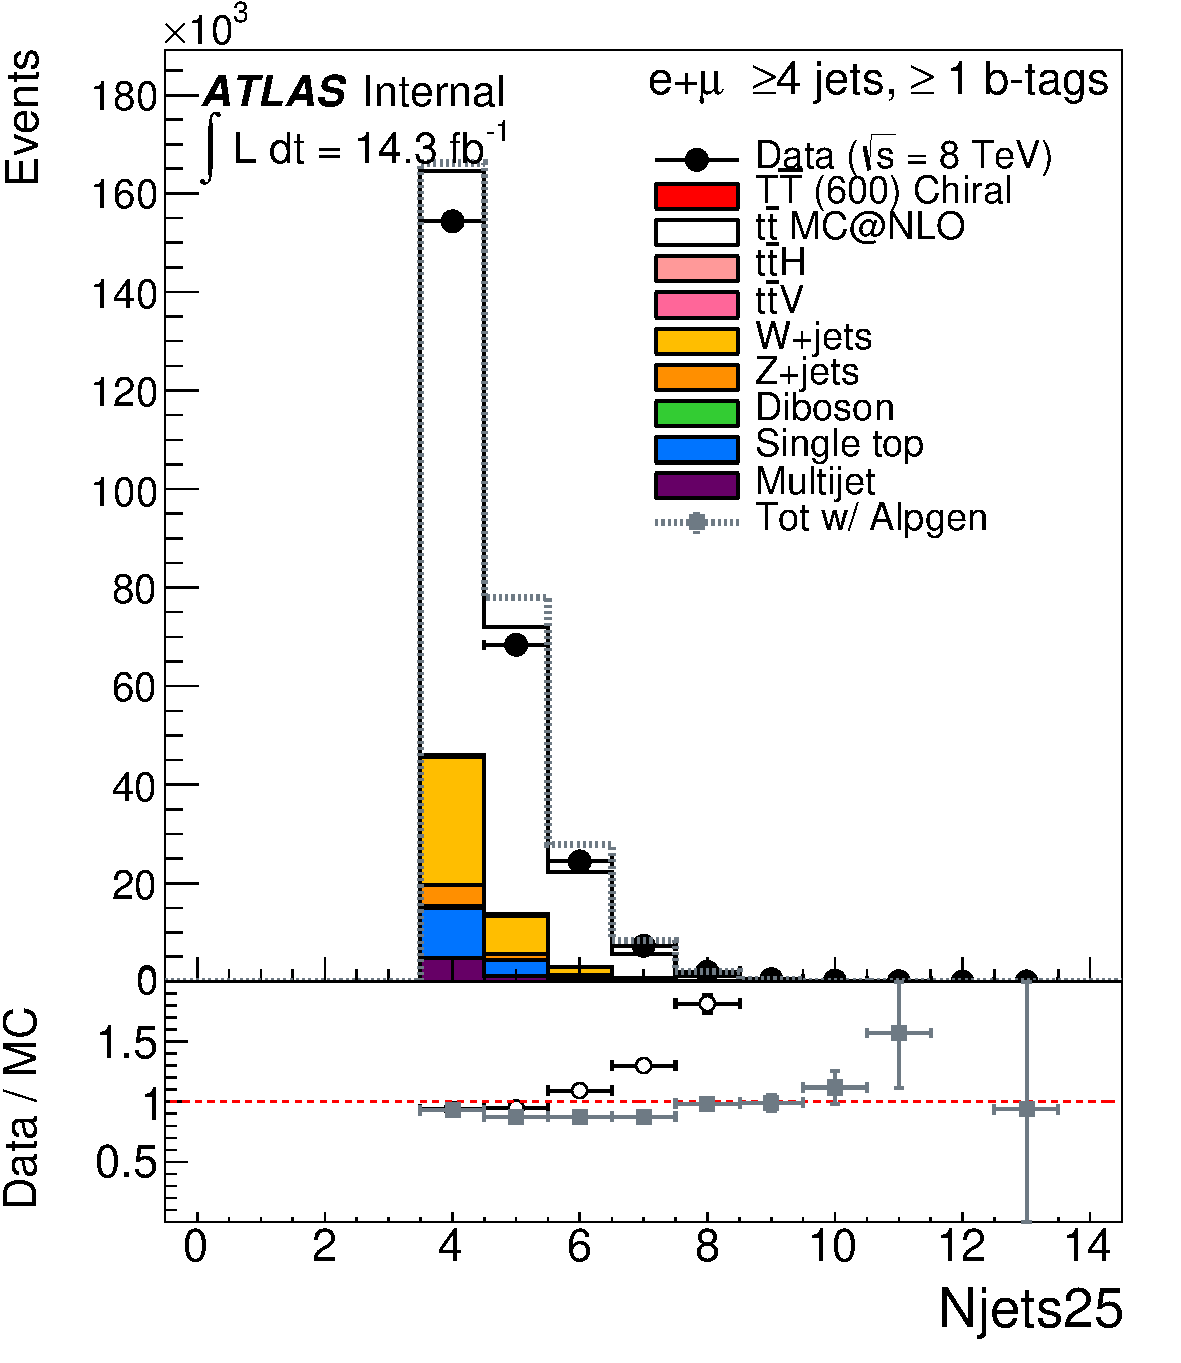
\includegraphics[width=0.32\textwidth]{vlq_analysis/figures/THESIS_c5_presel_noortho_noyields/ELEMUON/4jetin/1btagin/Njets25_ELEMUON_4jetin1btagin_NOMINAL}}
	%\subfigure[]{
  	%\includegraphics[width=0.32\textwidth]{vlq_analysis/figures/THESIS_c5_presel_noortho_noyields/ELEMUON/4jetin/1btagin/JetEta1_ELEMUON_4jetin1btagin_NOMINAL}}\\
	%\subfigure[]{
  	%\includegraphics[width=0.32\textwidth]{vlq_analysis/figures/THESIS_c5_presel_noortho_noyields/ELEMUON/4jetin/1btagin/nWhad_ELEMUON_4jetin1btagin_NOMINAL}}
	%\subfigure[]{
  	%\includegraphics[width=0.32\textwidth]{vlq_analysis/figures/THESIS_c5_presel_noortho_noyields/ELEMUON/4jetin/1btagin/Wlep_MassT_ELEMUON_4jetin1btagin_NOMINAL}}
	%\subfigure[]{
  	%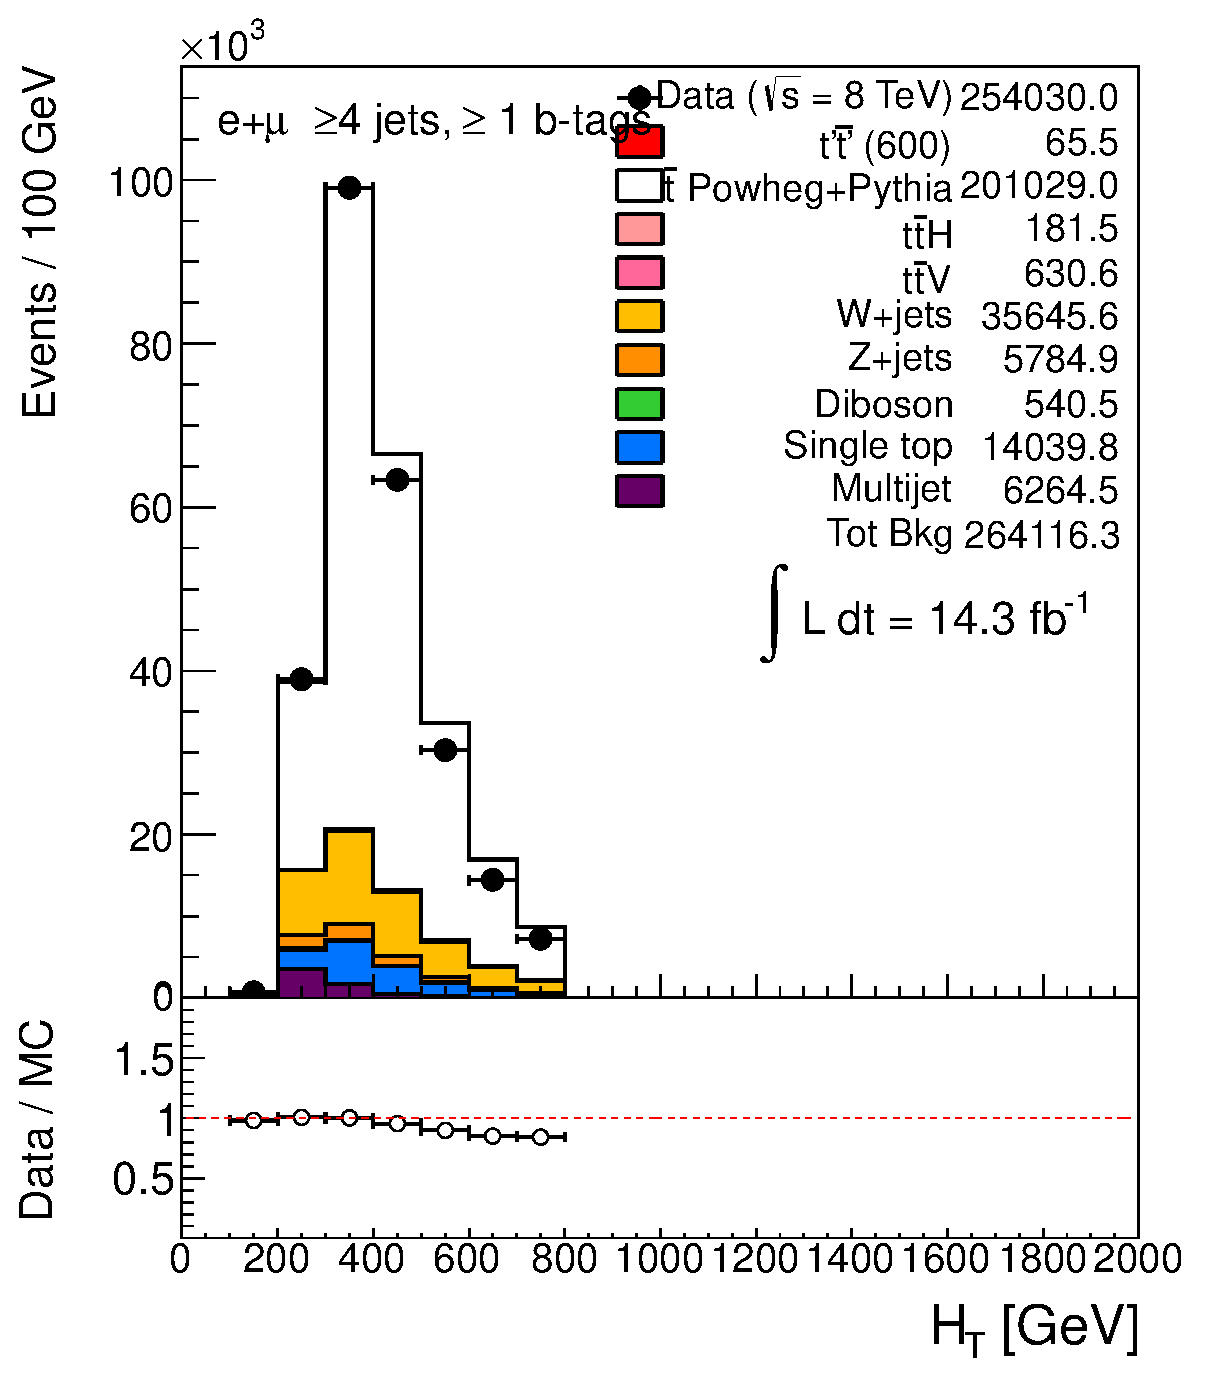
\includegraphics[width=0.32\textwidth]{vlq_analysis/figures/THESIS_c5_presel_noortho_noyields/ELEMUON/4jetin/1btagin/HTAll_ELEMUON_4jetin1btagin_NOMINAL}}
	\caption{Comparison between data and prediction plots for (a) lepton transverse momentum and
        (b) pseudorapidity, (c) missing tranverse energy, (d) transverse mass of $W$ boson, (e)
        leading jet transverse momentum, (f) number of jets with $\pt>25~\gev$.
        The selection is ``preselection'' with a blinding cut to reject signal on
        $\htfj<800\gev$. Systematic uncertainties are not shown.
        \label{fig:ELEMUON_4jetin1btagin}}
\end{center}\end{figure}



\section{Statistical analysis}\label{sec:cls}

To test the presence or absence of signals from new physics we use the
\cls{s} method~\cite{cls,cls_2}


\section{Systematic uncertainties}\label{sec:systematics}

In addition to the uncertainty that comes from the stocastical nature
of events we are subject to other sources that are systematical in the sense
that they will bias the result towards a definite direction. They can come from
detector measurements, from the way we reconstruct the objects, from the Monte
Carlo modelling, and can affect either only the normalization of the total event
yield (and are called ``normalization-only'' sytematics) or also the shape 
of the distributions (and are called ``shape and normalization'' systematics).

The individual sources of systematics are treated as uncorrelated, while
the correlations eventually present in the particual systematic uncertainty are 
kept for the various processes and channels. Most of the systematic uncertainties
are common to the two analyses presented with only minor differences, e.g. in the
\htx\  analysis the systematic uncertainty affecting the jet energy scale is
split into 9 components, while it has a unique component in the \wbx\  analysis. 
The full list of systematics considered is presented in 
Table~\ref{tab:SystSummary}, labelling them as  ``normalization-only'' 
or ``shape and normalization'' systematics and indicating the number of components.

\begin{table}[htb]
\centering
\begin{tabular}{lcccc}
\toprule
Systematic uncertainty & \multicolumn{2}{c}{ \wbx\  } & \multicolumn{2}{c}{ \htx\  }\\
 & Status  & Components & Status  & Components\\
\midrule
Luminosity                  &  N & 1 &  N & 1\\
Lepton ID+reco+trigger      &  N & 1 &  N & 1\\
Jet vertex fraction efficiency & SN & 1 & SN & 1\\
Jet energy scale            & SN & 1 & SN & 8\\
Jet energy resolution       & SN & 1 & SN & 1\\
%Jet mass scale               & - & -\\
%Jet mass resolution      & - & -\\
$b$-tagging efficiency      & SN & 9 & SN & 9\\
$c$-tagging efficiency      & SN & 5 & SN & 5\\
Light jet-tagging efficiency    & SN & 1 & SN & 1\\
$t\bar{t}$ cross section    &  N & 1 &  N & 1\\
$t\bar{t}V$ cross section   &  N & 1 &  N & 1\\
$t\bar{t}H$ cross section   & - & - &  N & 1\\
Single top cross section    &  N & 1 &  N & 1\\
Dibosons cross section      &  N & 1 &  N & 1\\
$W$+jets normalization      &  N & 5 &  - & -\\
$Z$+jets normalization      &  N & 1 &  - & -\\
$V$+jets normalization      &  - & - &  N & 1\\
Multijet normalization      &  - & - &  N & 1\\
$t\bar{t}$ modelling        & SN & 3 & SN & 3\\
$V$+jets modelling         & SN & 1 &  - & -\\
$t\bar{t}$+heavy-flavour fractions &  - & -& N & 1\\
%$\TT$ modelling        & - & -\\
\bottomrule
\end{tabular}
\caption{\label{tab:SystSummary} 
List of systematic uncertainties considered in the two analyses. 
We label as ``N'' (``SN'') uncertainties taken as ``normalization-only'' 
(both ``shape'' and ``normalization'')
for all processes and channels. 
Some of the systematic uncertainties are split into more 
components for a more
accurate treatment. }
\end{table}

The systematic uncertainties are treated inside the \mclimit\ 
package~\cite{mclimitATLAS} developed for ATLAS heavy quark
searches based on the original \mclimit\ code developed
by the CDF collaboration~\cite{Heinrich:7587,Junk:8128,Junk:7904}.
Here the  histograms are interpolated between the nominal and the 
systematically shifted templates bin-by-bin, with a shift of $+0.5\sigma$
corresponding to half way between the nominal and the $+1\sigma$ shifted template.
This interpolation method is called vertical morphing and uses a linear 
bin-by-bin interpolation, but for variations below $1\sigma$ we use
quadratic interpolation to ensure a continuous derivative at zero shift.
Pseudoexperiments are generated using these interpolated numbers for
all systematic uncertainties.

Details on specific treatments of systematics in particular channels will
be given in the dedicated sections of the corresponding analysis chapters 
(Section~\ref{sec:wbxSYS} and~\ref{sec:htxSYS}).



\subsection{Luminosity}
\label{sec:syst_lumi}
The uncertainty on the absolute integrated luminosity is estimated to be
of 3.6\%~\cite{lumi}. This systematic uncertainty
is applied to all processes except the QCD multi-jet background.

\subsection{Object definitions}
\label{sec:syst_objects}
The event reconstruction introduces uncertainties on the definition of
leptons, jets and on the $b$-, $c$-, and light flavour-tagging. In the
following the related systematic uncertainties considered are described.

\subsubsection{Lepton reconstruction, identification and trigger scale factors}
\label{sec:syst_lepID}

In Sections~\ref{sec:electrons} and~\ref{sec:muons} the reconstruction
of leptons was introduced, explaining the need of adjusting the
differences between data and simulation in the efficiency for
reconstruction, identification and trigger. This is done by
applying to Monte Carlo samples some scale factors derived 
with tag-and-probe techniques 
on $Z\to \ell^+\ell^-$ ($\ell=e,\mu$) data and simulated samples.
For each of these three sources of systematic uncertainty, 
the overall systematic uncertainty is obtained 
as the quadratic sum of the statistical
and systematic uncertainties on the corresponding scale factor.

In the $e$+jets channel, the systematic uncertainties corresponding to
electron reconstruction, identification and trigger, are 0.3\%, 1.1\% 
and 0.2\%, respectively.
In the $\mu$+jets channel, the systematic uncertainties corresponding to
muon reconstruction, identification and trigger, are 0.2\%, 1.1\% and 1.4\%, 
respectively.
A total uncertainty on the signal and background acceptances of 2\% is estimated.


\subsubsection{Lepton momentum scale and resolution}

To check the accuracy of the lepton momentum scale and resolution
simulated samples of $Z\to \ell^+\ell^-$ and $J/\psi \to \ell^+\ell^-$
are used to reconstruct the particles masses (for electrons also
 $W\to e\nu$ events are used from  $E/p$  studies).
The small discrepancies observed between data and simulation are
corrected adjusting lepton energy scale and resolution in Monte Carlo
samples only for muons, while for electrons energy resolution corrections
are also applied only to Monte Carlo samples but energy scale corrections
are applied to data in all detector regions and to simulation only in 
the calorimeter transition region.
The systematic uncertainties on these scale factors are varied
separately and the result on the total yields are are at the 
sub-percent level and considered therefore ngligible in the analyses.

\subsubsection{JVF efficiency}
\label{sec:syst_jvf}

Recalling the cut applied on the JVF variable (Section~\ref{sec:jets}) 
of $|{\rm JVF}|>0.5$, the per-jet efficiency of this requirement
is estimated in $Z(\to \ell^+\ell^-)$+1-jet events both in data and
Monte Carlo simulation. Event enriched in hard-scatter jets are selected
separately from events enriched in jets from pile-up interactions and
specific efficiency and inefficiency scale factors are measured.
Scale factors for pileup jets are estimated to be consistent with 1, while
efficiency for hard-scatter jets goes from $\sim$1.03 for jets with $\pt=25\gev$
down to $\sim$1.01 for jets with $\pt>150\gev$.
An overall event weight is obtained as the product of all per-jet scale factors
and is applied to the Monte Carlo samples.
The systematic uncertainty from the propagation of the per-jet scale
factor uncertainty gives an overall uncertainty on the signal
and background acceptance of $\sim$2.5\%.


\subsubsection{Jet energy scale}
\label{sec:syst_jes}

The systematic uncertainty on the Jet Energy Scale (JES) 
has been derived combining the information from both test-beam 
and collision data and Monte Carlo
simulation~\cite{ATLASJetEnergyMeasurement, insitu5,insitu6}.  
Pile-up activity produces an additional source of systematic 
uncertainty which depends on the number of primary vertices
and on the average number of interactions per bunch crossing $<\mu>$. 
%The first estimate of the effect of pile-up on the jet energy scale uncertainty was developed in 2011~\cite{insitu6}, and subsequently validated with in situ momentum balance techniques in studies of the 2012 data.
Momentum balance techniques in $Z$+jets, $\gamma$+jets and 
multi-jet events are combined to derive a small residual correction
for jets in the transverse momentum range $20\gev<\pt<\sim1\tev$.

The overall variation due to JES systematic uncertainty 
evaluated in the central detector region 
is $\sim$4\% for jets with $\pt=25\gev$ and improves to $\sim$1\% for  
jets with $\pt=500\gev$~\cite{jesuncertainty}.
The effect of this systematic uncertainty is 
implemented in the analyses by varying in the Monte Carlo samples the 
transverse momentum of all the selected jets by $\pm$1 standard deviation.
In each event the missing transverse momentum \met\ is then corrected consistently to 
the varied $\pt$ of the jets and all the variables involving jets are also
recomputed.

As can be seen in Table~\ref{tab:SystSummary}, for the \htx\ analysis
the JES systematic uncertainty is split into 8
uncorrelated components, each with a different jet $\pt$ and $\eta$
dependence, which are treated independently.
The \wbx\ instead uses the total JES uncertainty as a single uncertainty
resulting from the sum in quadrature of all individual sources.



\subsubsection{Jet energy resolution}
\label{sec:syst_jer}

The Jet Energy Resolution (JER) was measured 
with two {\em in-situ} techniques~\cite{ATLASJetEnergyMeasurement}
as a function of the jet transverse momentum and pseudo-rapidity.
It is consistent in data and Monte Carlo simulation and no corrections
are needed.
To account for the systematic uncertainty the quadratic difference 
between the JER in data and in simulated samples is used
to smear the energy of jets in Monte Carlo simulation and a new
varied sample is obtained with a different normalisation and 
variable distributions shapes. The final result is then symmetrised
to obtain both positive and negative variations.
%In order to propagate the uncertainty in the $\pt$ resolution, for each jet in the simulation, a random number $r$ is drawn from a Gaussian distribution with mean 0 and sigma equal to the difference in quadrature between the fractional $\pt$ resolution with the tool and the nominal one.  The jet 4-momentum is then scaled by a factor $1+r$. This jet energy resolution uncertainty is assumed to be fully correlated point-by-point.
%The same rebinning algorithm as discussed in Section~\ref{sec:syst_jes} is applied.


\subsubsection{Heavy- and light-flavour tagging}
\label{sec:syst_btag}


The efficiencies in heavy flavour ($b$ and $c$) jets identification with
the $b$-tagging algorithm are measured in data and depend on the individual
jet flavour~\cite{BTaggingEfficiency,CTaggingEfficiency,LightTaggingEfficiency}.
These efficiencies are measured from data and depend on the jet flavour:
in Monte Carlo events $b$ ($c$) jet efficiencies are corrected with scale factors
of 0.9--1.0 (1.1--1.2) depending on $\pt$, light jet efficiencies are corrected 
with a  scale factor of $\sim$1.3.
Every jet in the Monte Carlo simulated events is corrected depending
on its flavour, $\pt$ and $\eta$
The uncertainty on these scale factors is 
between 7\% and 13\% for $b$ jets, between 15\% and 39\% for $c$ jets,
and $\sim$25\% for light jets.

As was reported in Table~\ref{tab:SystSummary}, the systematic uncertainty
on \btag ging (\ctag ging) efficiency is divided into nine (five) independent 
components that correspond to an eigenvector from the diagonalization of the
matrix containing the information on the total uncertainty 
per $\pt$ bin and the bin-to-bin correlations (see~\cite[Appendix P]{VHbb} for
more details).
These individual sources of systematic uncertainties 
are taken as uncorrelated between $b$, $c$ jets, and
light flavour jets. In Monte Carlo simulated events 
a per-jet weighting procedure~\cite{IFAEBtagNote}
is applied in order to propagate the \btag ging calibration
and related uncertainties.

\subsection{Theoretical cross-sections}
\label{sec:syst_bkgxsect}

Normalization-only systematic uncertainties on the theoretical
cross-sections are considered as follows:
+10\%/-11\% for the inclusive $t\bar{t}$
production cross section evaluated at approximate NNLO using 
\texttt{HATHOR}~\cite{ttbarxs}; +5\%/-4\% and $\pm 5\%$ 
for the theoretical cross sections of the single
top~\cite{stopxs,stopxs_2} and diboson~\cite{dibosonxs} backgrounds
respectively; +12\%/-17\% and  $\pm 30\%$ 
for the theoretical cross sections of the $t\bar{t}H$~\cite{lhcxs} and 
$t\bar{t}V$~\cite{ttbarVxs1,ttbarVxs2} backgrounds respectively.


\subsection{Normalizations of data-driven backgrounds and background modeling}
\label{sec:syst_norm}

Because of the differences between the effects of these systematic uncertainties
in the \wbx\ and \htx\ analyses, the reader is referred to the specific 
Sections~\ref{sec:wbxSYS} and~\ref{sec:htxSYS}


%
\section{Search for \TTbar\ pairs decaying to $Wb+X$}\label{sec:wbx}

\subsection{Boosted $W$ reconstruction}\label{subsec:boostedW}

\subsection{Control regions}\label{sec:wbxCR}

\subsection{Event selection}\label{sec:wbxEVT}

%\subsection{}\label{sec:}

%\subsection{}\label{sec:}

\subsection{Systematics}\label{sec:wbxSYS}

%
\section{Preliminary search for \TTbar\ pairs decaying to $Ht+X$}\label{sec:htx}

\subsection{Control regions}\label{sec:htxCR}

\subsection{Event selection}\label{sec:htxEVT}

%\subsection{}\label{sec:}

%\subsection{}\label{sec:}

\subsection{Systematics}\label{sec:htxSYS}

